\documentclass{article}

\usepackage[a4paper, total={6in, 8in}]{geometry}
\usepackage[english, lithuanian]{babel}
\usepackage{float}
\usepackage{amsmath}
\usepackage{subcaption}
\usepackage{datetime}
\usepackage{comment}
\usepackage{caption}
\usepackage{graphicx}
\usepackage{amsfonts}
\usepackage{listings}
\usepackage{amssymb}
\usepackage[T1]{fontenc}
\usepackage{url}
\usepackage{xcolor}

\DeclareUnicodeCharacter{2212}{-}
\selectlanguage{lithuanian}

\definecolor{backcolour}{rgb}{0.95,0.95,0.92}
\definecolor{codegreen}{rgb}{0,0.6,0}

\lstdefinestyle{myStyle}{
    backgroundcolor=\color{backcolour},   
    commentstyle=\color{codegreen},
    basicstyle=\ttfamily\footnotesize,
    breakatwhitespace=false,         
    breaklines=true,                 
    keepspaces=true,                 
    numbers=left,       
    numbersep=5pt,                  
    showspaces=false,                
    showstringspaces=false,
    showtabs=false,                  
    tabsize=2,
}
\lstset{style=myStyle}

\begin{document}
\newlength{\mywidth}
\settowidth{\mywidth}{Darbo vadovas:}
\begin{titlepage}
    \vskip 20pt
    \centerline{\bf \large VILNIAUS UNIVERSITETAS}
    \bigskip
    \centerline{\large \textbf{MATEMATIKOS IR INFORMATIKOS FAKULTETAS}}
    \vskip 120pt
    \centerline{\bf \Large \textbf{Laboratorinis darbas 1}}
    \vskip 50pt
    \begin{center}
        {\bf \LARGE Vienmatis optimizavimas}
    \end{center}
    \bigskip
    \bigskip
    \centerline{\Large Nikita Gainulin}
    \vskip 90pt
    \vskip 200pt
    \centerline{\large \textbf{VILNIUS 2024}}
\end{titlepage}

\tableofcontents

\clearpage
\section{Tikslo funkcija}
Visi šioje ataskaitoje minėti metodai bus pritaikyti šiai tikslo funkcijai:
\begin{equation}\label{eq:1}
    f(x) = \frac{(x^2-5)^2}{7}-1
\end{equation}
Mano \textit{Python} kode aprašyta taip:
\lstinputlisting[language=Python]{fx.py}
\section{Vienmačiai optimizavimo metodai ir jų algoritmų kodai}
\subsection{Intervalo dalijimo pusiau metodas}
Pirmiausia reikia nustatyti intervalą, kuriame ieškosime minimumo taško. Minėto intervalo ribas įsiminsime kintamaisiais \textit{l} (kairioji riba) ir \textit{r} (dešinioji riba). Pradiniame intervale pasirenkam tris bandymo taškus $x_{1}$, $x_{2}$ ir $x_{m}$, taip, kad $x_{m}$ būtų intervalo vidurio taškas, o $x_{1}$ ir $x_{2}$ tarp \textit{l} ir vidurio taško bei \textit{r} ir vidurio taško atitinkamai. Tada apskaičiuojame $f(x_{m})$, $f(x_{1})$ ir $f(x_{2})$ reikšmes. Po to palyginame gautas reikšmes, t. y. kuriame taške funkcija įgyja didesnę reikšmę. Tas taškas ir nustato intervalą, kurį reikia atmesti. Kadangi ieškome minimumo taško, atmetamas atitinkamas intervalas, atitinkmai keičiami $x_{1}$, $x_{2}$ ir $x_{m}$ taškai bei perskaičiuojami $f(x_{m})$, $f(x_{1})$ ir $f(x_{2})$ reikšmės. Algoritmas tęsiamas tol, kol gaunamas pakankamai tikslus minimumo taškas, t.y. kol intervalo ilgis $r-l$ nėra mažiau už tam tikrą $\varepsilon$ reikšmę.\\
Štai kaip tai atrodo mano \textit{Python} kode:
\lstinputlisting[language=Python]{halfcut.py}
Vizualizuojant mūsų tikslo funciją (\ref{eq:1}) šiuo metodu gauname štai tokį grafą:
\begin{figure}[H]
    \centering
    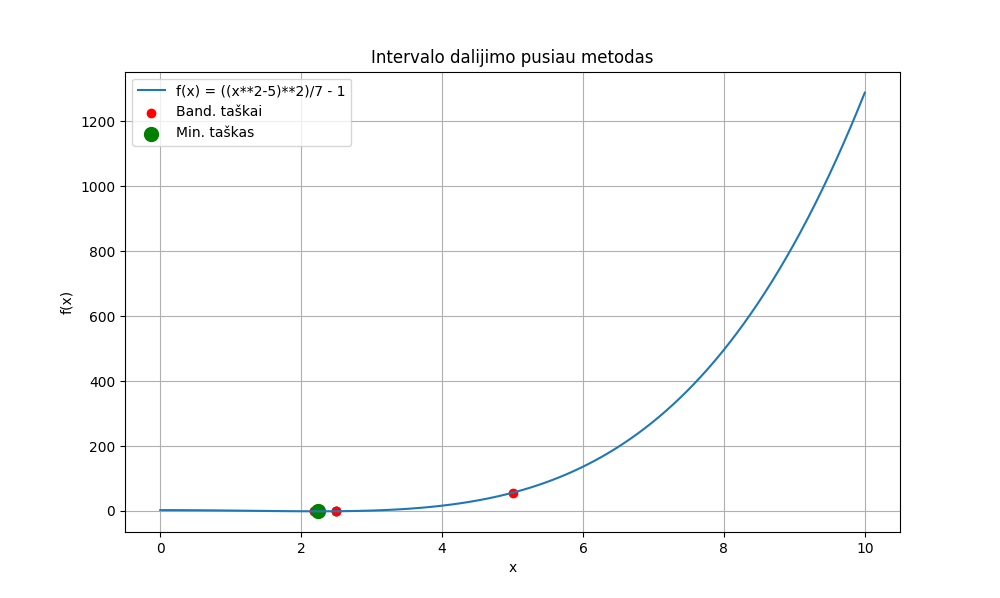
\includegraphics[width=1\textwidth]{Figure_1.png}
    \caption{Intervalo dalijimo pusiau metodo vizualizacija (\ref{eq:1}) tikslo funkcijai.}
    \label{fig:1}
\end{figure}
\subsection{Auksinio pjūvio metodas}
Šis metodas yra labai panašus į intervalo dalijimo pusiau metodą, tačiau per kiekvieną iteraciją naudojami tik 2, o ne 3 bandomieji taškai. Mums vis dar reikia pasirinkti intervalą ir įsiminti jo kairiąją \textit{l} ir dešiniąją \textit{r} ribas, tačiau šį kartą $x_{1}$ ir $x_{2}$ apskaičiuojami kitaip, naudojant \textit{Fibonačio} reikšmę, kuri apytiksliai lygi:
\begin{equation*}
    \tau = \frac{\sqrt{5}-1}{2} \approx 0.61803...
\end{equation*}
Apskaičiavę $x_{1}=r-\tau(r-l)$ ir $x_{2}=l+\tau(r-l)$ taškus, apskaičiuojame funkcijos reikšmes $f(x_{1})$ ir $f(x_{2})$ šiuose taškuose. Po to dar kartą palyginame funkcijos reikšmes ir pašaliname intervalus pagal didesnę vertę, perskaičiuojame taškus ir naujas funkcijos reikšmes ir kartojame tuos pačius veiksmus kiekvieną iteraciją, kol vėl gauname pakankamai tikslų minimumo tašką.\\
Algoritmo \textit{Python} kodas:
\lstinputlisting[language=Python]{goldratio.py}
Vizualizuojant mūsų tikslo funciją (\ref{eq:1}) šiuo metodu gauname štai tokį grafą:
\begin{figure}[H]
    \centering
    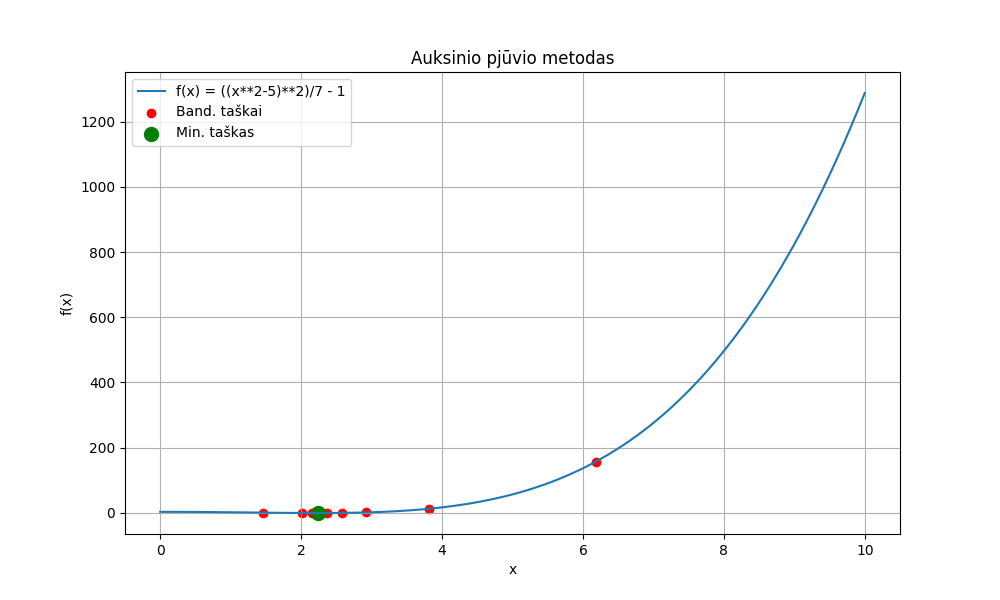
\includegraphics[width=1\textwidth]{Figure_2.png}
    \caption{Auksinio pjūvio metodo vizualizacija (\ref{eq:1}) tikslo funkcijai.}
    \label{fig:2}
\end{figure}
\subsection{Niutono metodas}
Skirtingai nuo dviejų ankstesnių metodų, kurie remiasi konkretaus intervalo pjovimu, Niutono metodas remiasi vienu pradiniu tašku $x_{i}$ ir Teiloro eilutėmis iki antros eilės. Pasirinkus pradinį tašką $x_{i}$, kitas taškas apskaičiuojamas pagal šią formulę:
\begin{equation}\label{eq:2}
    x_{i+1} = x_{i} - \frac{f'(x_{i})}{f''(x_{i})}
\end{equation}
Tokiu būdu iteracija po iteracijos taškas artėja prie minimumo.\\
Vienas įdomus faktas, kurį pastebėjau, yra tai, kad daugelyje internetinių šaltinių kaip Niutono metodo pagrindas naudojama ši formulė:
\begin{equation*}
    x_{i+1} = x_{i} - \frac{f(x_{i})}{f'(x_{i})}
\end{equation*}
Nors ši formulė paprastai naudojama dažniau ir bendriau, formulė (\ref{eq:2}) yra tikslesnė optimizavimo kontekste, todėl ją ir naudojame vietoj šios bendrosios formulės.\\
Algoritmo \textit{Python} kodas:
\lstinputlisting[language=Python]{newton.py}
Vizualizuojant mūsų tikslo funciją (\ref{eq:1}) šiuo metodu gauname štai tokį grafą:
\begin{figure}[H]
    \centering
    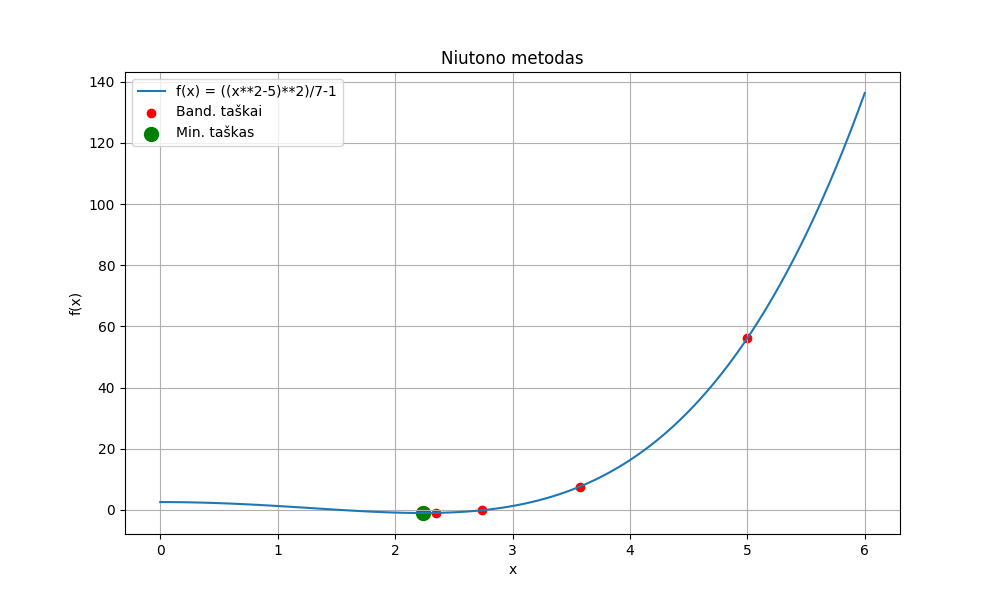
\includegraphics[width=1\textwidth]{Figure_3.png}
    \caption{Niutono metodo vizualizacija (\ref{eq:1}) tikslo funkcijai.}
    \label{fig:3}
\end{figure}
\section{Rezultatai ir jų palyginimai}
\subsection{Minimumo taškas ir funkcijos reikšmė tame taške}
Kaip ir galima tikėtis, taikant visus metodus gaunami daugiau ar mažiau panašūs rezultatai, kai kalbama apie minimumo tašką:
\begin{table}[H]
    \centering
    \begin{tabular}{|p{3cm}|p{3cm}|p{3cm}|p{3cm}|}
    \hline
    \multicolumn{1}{|l|}{} & Intervalo dalijimo pusiau metodas & Auksinio pjūvio metodas & Niutono metodas \\ \hline
                       Minimumo taškas    & 2.236061 & 2.236057 & 2.236105 \\ \hline
                       F-jos reikšmė   & -0.999999 & -0.999999 & -0.999999 \\ \hline
    \end{tabular}
\end{table}
Matomas šiek tiek didesnis Niutono metodo nuokrypis nuo kitų metodų. Tačiau tai nebūtinai yra blogai, tiesiog rodo, kad Niutono metodo tikslumas priklauso nuo tokių parametrų kaip pradinis taškas ir funkcijos pobūdis.

\end{document}